\documentclass[main]{subfiles}


\title[AutoML in the Age of Foundation Models]{AutoML in the Age of Foundation Models}
\subtitle{The Big Picture}
\author[Marius Lindauer]{Marius Lindauer}
\date{}

\titlebackground*{images/AutoML_Agentic}

%\institute{}
%\date{}

\begin{document}
	
	\maketitle
	

%----------------------------------------------------------------------
%----------------------------------------------------------------------
\begin{frame}[c]{What are Foundation Models?}

\centering
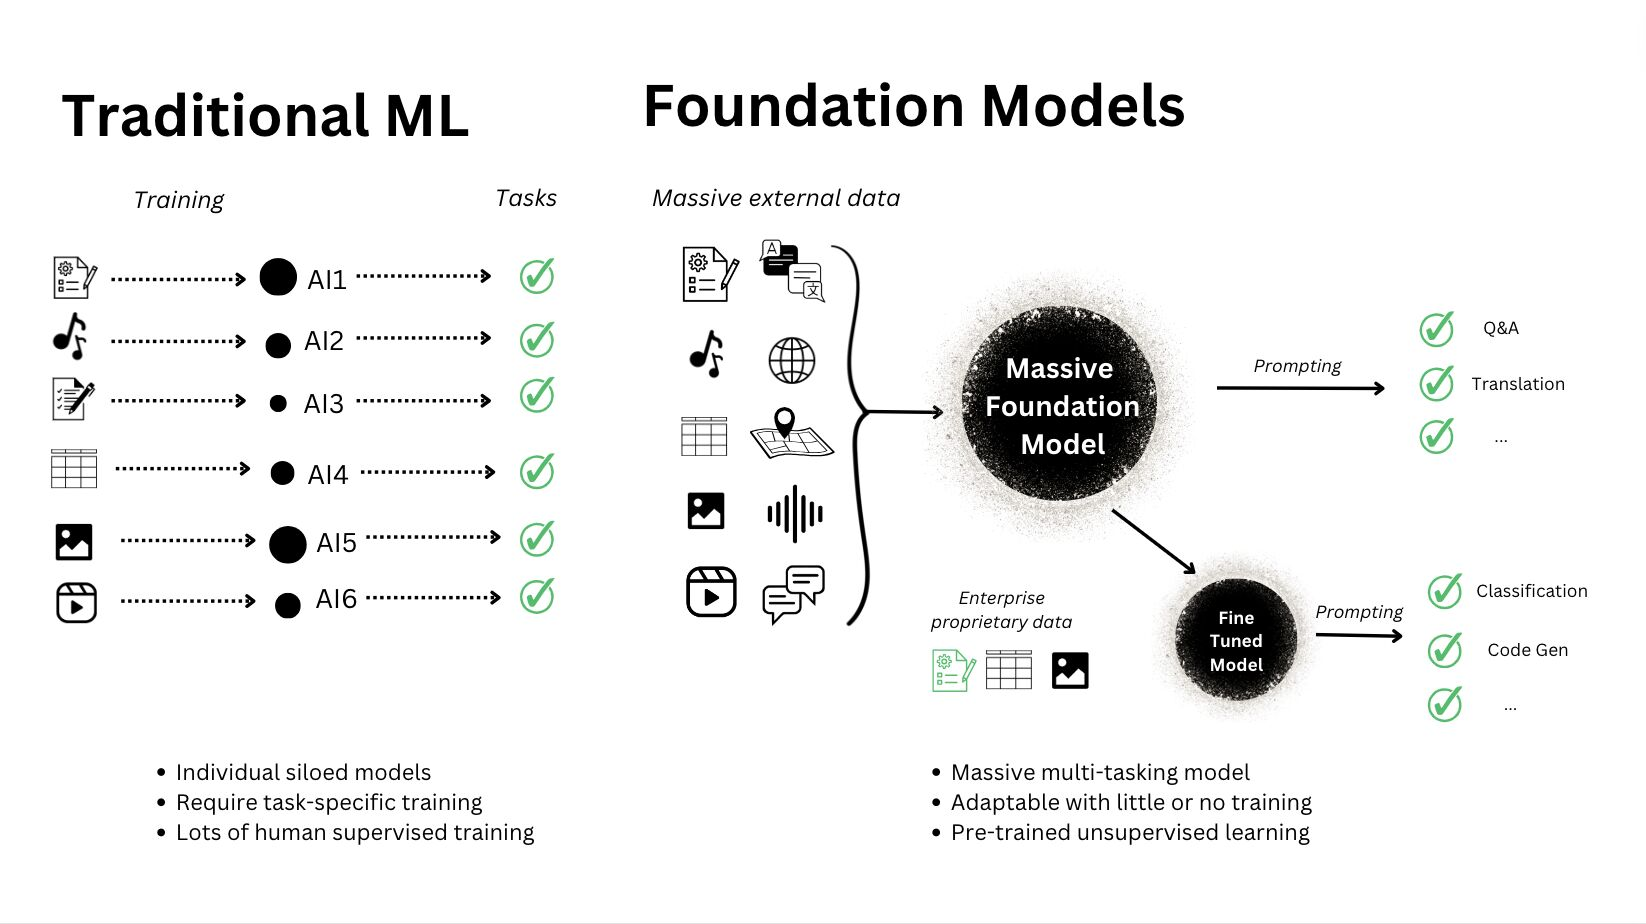
\includegraphics[width=0.7\textwidth]{images/foundation-models-explained.jpeg}

\liturl{Armand Ruiz| Conor Kelly}{https://humanloop.com/blog/foundation-models}

\end{frame}
%-----------------------------------------------------------------------
%----------------------------------------------------------------------
\begin{frame}[c]{Why are Foundation Models a Challenge for AutoML? \liturl{Tornede et al. 2024}{https://arxiv.org/abs/2306.08107}}

\centering
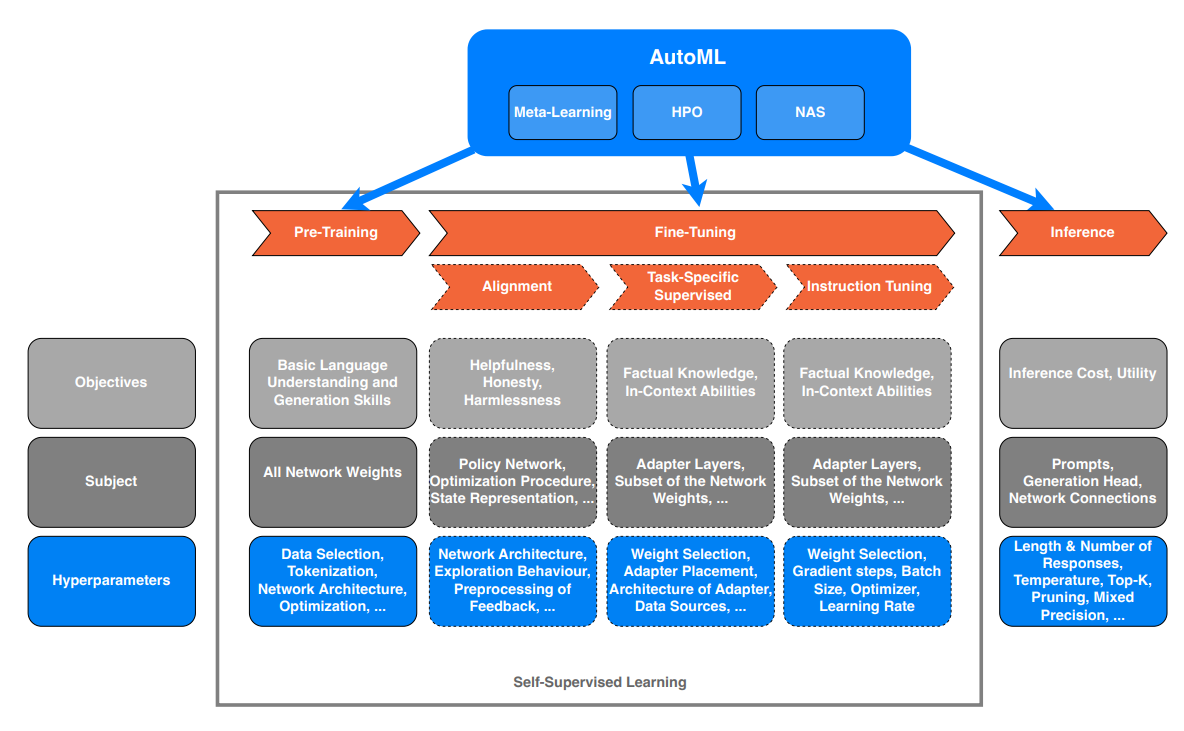
\includegraphics[width=0.7\textwidth]{images/automl_llms}

\end{frame}
%-----------------------------------------------------------------------
%----------------------------------------------------------------------
\begin{frame}[c]{Why are Foundation Models a Challenge for AutoML? \liturl{Tornede et al. 2024}{https://arxiv.org/abs/2306.08107}}

\begin{itemize}
    \item Foundation models require very expensive pre-training\\ $\leadsto$ training many ($n > 10$) models with different settings is basically infeasible 
    \item Training foundation models often combines several learning paradigms, e.g., self-supervised learning, supervised learning and reinforcement learning\\
    $\leadsto$ Each of them comes with its own metric and design spaces\\
    $\leadsto$ There are interactions between stages, but, so far, they have to be tuned independently
    \item Foundation models make use of several data modalities (e.g., text, images, and videos)\\
    $\leadsto$ Each of them comes also with their own data preprocessing and backbone models
\end{itemize}

\end{frame}
%-----------------------------------------------------------------------
%----------------------------------------------------------------------
\begin{frame}[c]{What are new Opportunities Thanks to Foundation Models?}

\begin{itemize}
    \item Foundation models can be trained for AutoML tasks \liturl{Chen et al. 2022}{https://arxiv.org/abs/2205.13320} \liturl{Müller et al 2023}{https://arxiv.org/abs/2305.17535}
    \item LLMs are the most powerful meta-models to date, allowing access to prior knowledge from all kinds of sources (books, papers, tutorials, code, etc pp)
    \item LLMs can (more easily) operate in unbounded spaces, e.g., in contrast to the typical bounded spaces of BO for HPO, which (potentially) require expert knowledge to define the spaces before using AutoML techniques
    \item LLMs (and agentic systems) allow for the generation of code, vastly increasing the scope of AutoML down to the code level
\end{itemize}

\end{frame}
%-----------------------------------------------------------------------


\begin{frame}{Summary} 

Most important insights from this video:

\begin{enumerate}
    \item It's an exciting time to see how AutoML flourishes and faces new challenges at the same time
    \item AutoML is going to be redefined from narrow tasks to broader and more powerful capabilities
\end{enumerate}

$\leadsto$ We will focus on new possibilities for AutoML enabled by foundation models, LLMs, and agentic systems in the next videos.

\end{frame}

\end{document}
